%%% LaTeX Template: Article/Thesis/etc. with colored headings and special fonts
%%%
%%% Source: http://www.howtotex.com/
%%% Feel free to distribute this template, but please keep to referal to http://www.howtotex.com/ here.
%%% February 2011
%%%
%%% Modified January 2016 by CDM

%%%  Preamble
\documentclass[11pt,letterpaper]{article}
\usepackage[margin=1.0in]{geometry}
\usepackage[T1]{fontenc}
\usepackage[bitstream-charter]{mathdesign}
\usepackage[latin1]{inputenc}					
\usepackage{amsmath}						
\usepackage{xcolor}
\usepackage{cite}
\usepackage{hyphenat}
\usepackage{graphicx}
\usepackage{float}
\usepackage{subfigure}
\usepackage{sectsty}
\usepackage[compact]{titlesec} 
\usepackage[tablegrid]{vhistory}
\usepackage{pbox}
\allsectionsfont{\color{accentcolor}\scshape\selectfont}

%%% Definitions
\definecolor{accentcolor}{rgb}{0.0,0.0,0.5} 
\newcommand{\teamname}{Team Name}
\newcommand{\productname}{RFID Automated Student Pickup}
\newcommand{\coursename}{CSE 4317: Senior Design II}
\newcommand{\semester}{Spring 2018}
\newcommand{\docname}{Detailed Design Specification}
\newcommand{\department}{Department of Computer Science \& Engineering}
\newcommand{\university}{The University of Texas at Arlington}
\newcommand{\authors}{Bibek Khatakho \\ Austin Hastings \\ Kashif Iqbal \\ Nupur Pandey \\ Albaro Tonoco}

%%% Headers and footers
\usepackage{fancyhdr}
	\pagestyle{fancy}						% Enabling the custom headers/footers
\usepackage{lastpage}	
	% Header (empty)
	\lhead{}
	\chead{}
	\rhead{}
	% Footer
	\lfoot{\footnotesize \teamname \ - \semester}
	\cfoot{}
	\rfoot{\footnotesize page \thepage\ of \pageref{LastPage}}	% "Page 1 of 2"
	\renewcommand{\headrulewidth}{0.0pt}
	\renewcommand{\footrulewidth}{0.4pt}

%%% Change the abstract environment
\usepackage[runin]{abstract}			% runin option for a run-in title
%\setlength\absleftindent{30pt}			% left margin
%\setlength\absrightindent{30pt}		% right margin
\abslabeldelim{\quad}	
\setlength{\abstitleskip}{-10pt}
\renewcommand{\abstractname}{}
\renewcommand{\abstracttextfont}{\color{accentcolor} \small \slshape}	% slanted text

%%% Start of the document
\begin{document}

%%% Cover sheet
{\centering \huge \color{accentcolor} \sc \textbf{\department \\ \university} \par}
\vspace{1 in}
{\centering \huge \color{accentcolor} \sc \textbf{\docname \\ \coursename \\ \semester} \par}
\vspace{0.5 in}
\begin{figure}[h!]
	\centering
   	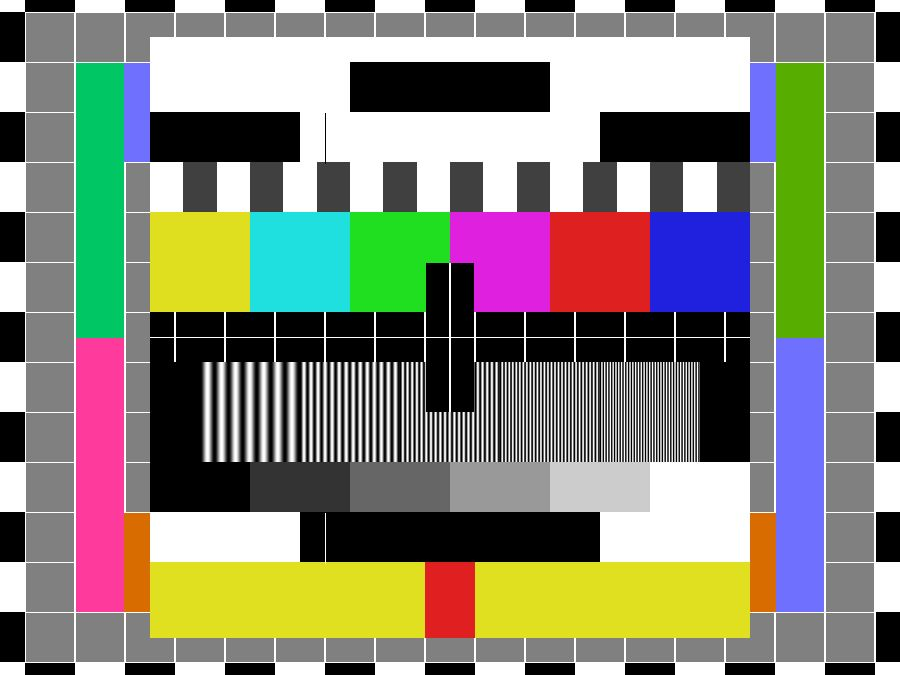
\includegraphics[width=0.60\textwidth]{images/test_image}
\end{figure}
\vspace{0.5 in}
{\centering \huge \color{accentcolor} \sc \textbf{\teamname \\ \productname} \par}
\vspace{0.5 in}
{\centering \large \sc \textbf{\authors} \par}
\newpage


%\vspace{1 in}
%\centerline{January 13th, 2012}
%\newpage

%%% Revision History
\begin{versionhistory}
  	\vhEntry{0.1}{2.23.2018}{AT|AH}{document creation}
\end{versionhistory}
\newpage

%%% Table of contents
\setcounter{tocdepth}{2}
\tableofcontents
\newpage

%%% List of figures and tables (optional)
\listoffigures
\listoftables
\newpage

%%% Document sections
\section{Introduction}
The project will be able to automate student pickup from school. Parents or guardians need to
have a tag that will be read by RFID reader. From the RFID reader the school staffs shall be able to get
the name and other information of the students. This shall expedite the process of student pickup as
now parents are using a piece of paper to pick up their kids. Initial versions of the system will use a
wire tether for data transfer between the RFID and processing unit. The majority of processing will be
accomplished by RFID and processor.

\section{System Overview}
\quad \quad The overall structure of the software system contains three layers: Student Management 
System, DataBase, and Queue Display System. The Student Management System is user end 
system which is related to administrative functionality that includes adding, removing 
and editing student and staff information in the system. The GUI allows the admin to 
add student and remove student. The DataBase System is responsible for storing the 
information. It also allows the user to make queries. The Queue Display System displays 
the information of the system and also handles the RFID listener. This is a user end 
system and also includes hardware. The Queue Display System and Database System 
communicate with each other to keep real time records of the student pickup.

\begin{figure}[h!]
	\centering
 	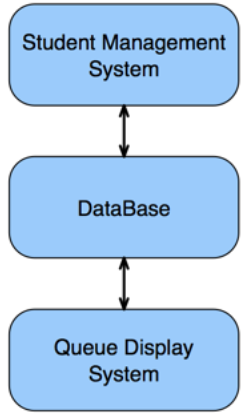
\includegraphics[width=0.40\textwidth]{images/ads_1}
 \caption{Overall Structure of System}
\end{figure}

\subsection{Student Management System Layer Description}
\quad \quad The Student Management System includes a control system, database control, and GUI. 
Control. This System directly talks with the Database System in order to store all the 
information about the students.

\subsection{Database Layer Description}
\quad \quad This System contains the tables to store the text and image of the system. Database 
System directly talks with Student Management System and Queue Display System.

\subsection{Queue Display System Layer Description}
\quad \quad This System contains control system, dbcontrol, GUI and RFID API. The RFID API helps 
to maintain communication between the Queue Display System and the RFID reader. The 
GUI displays the list of the students as their parents approach the school.
\newpage
%\section{Subsystem Definitions \& Data Flow}
%\quad \quad Will update this section later.

\begin{figure}[h!]
	\centering
 	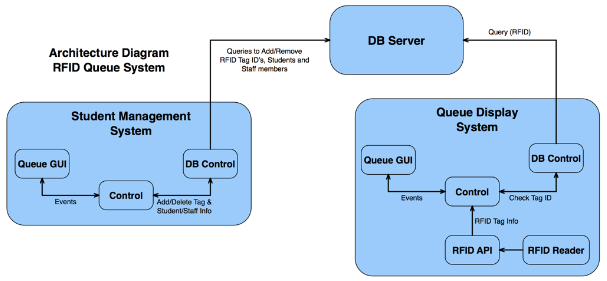
\includegraphics[width=0.9\textwidth]{images/ads_2}
 \caption{Data Flow Diagram}
\end{figure}

\newpage
\section{X Layer Subsystems}
	This subsystem will make various queries to the database as RFID tags become ready and display
all the associated data to the Queue GUI.

\subsection{Layer Hardware}
RFID integrated readers by Chafon Technology co. This system requires the hardware to begin the process of scanning tags. The two RFID readers are attached to two 8ft speaker tripods by Pyle. The RFID readers are connected in two ways. 1st: To a 9v/3A AC adapter to supply the readers power source,  2nd: A 10ft serial connection to usb for the reader to send the data back to the server for processing the RFID tags. 

\subsection{Layer Operating System}
Windows 10 

\subsection{Layer Software Dependencies}
Chafon Technology co. provided the base C# API for the reader, modified to render tags in a readable format. 

\subsection{Subsystem 1}
This system has a single one-way interface, it parses the RFID tag from the reader into a format
that the Control system can use.

\begin{figure}[h!]
	\centering
 	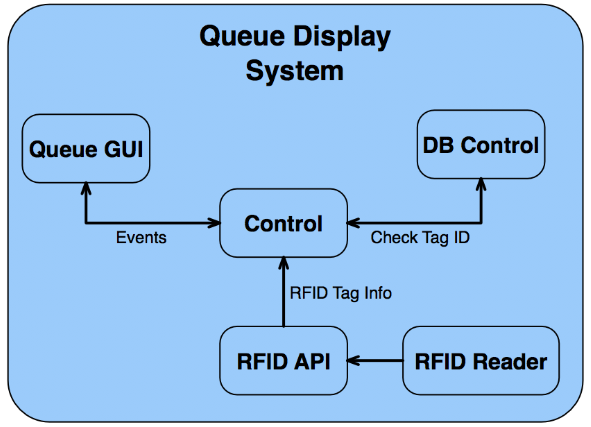
\includegraphics[width=0.60\textwidth]{images/ads_4}
 \caption{Queue Display Subsystems}
\end{figure}

\subsubsection{Subsystem Hardware}
This subsystem will identify the RFID tag that is scanned from the RFID Reader, utilizing the RFID
API it will send the data to the Control model.

\subsubsection{Subsystem Operating System}
Windows 10

\subsubsection{Subsystem Software Dependencies}
C# Chafon RFID API


\subsubsection{Subsystem Data Structures}
HTTP message once the tag id has been read is broadcast to local host. Checking the Database if the tag matches the DB will retrieve the associated data to the queue gui 





\newpage
\section{Y Layer Subsystems}
This subsystem communicates and controls database and Graphical user interface. This is needed
for setting up the initial database for all the users, admin, students, etc.

\subsection{Layer Operating System}
Windows 10

\subsection{Layer Software Dependencies}
Python pyqt4 module 

\subsection{Queue GUI subsystem}
This subsystem will talk with the control subsystem and displays the list of the names of students
in the GUI. This system has two, two-way interfaces. The first is directly connected to the computer recieving
keyboard and mouse input and relaying to the screen. The second passes and receives from Control.

\begin{figure}[h!]
	\centering
 	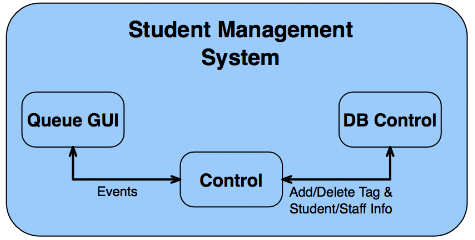
\includegraphics[width=0.60\textwidth]{images/ads_3}
 \caption{Student Management Subsystem}
\end{figure}


\subsubsection{Subsystem Programming Languages}
python subsystem programming language

\subsection{DB Control subsystem}
This subsystem handles all the data related to students needing to be dismissed by staff. This is the
subsystem that handles forwarding and receiving information from the database. This system has two, two-way interfaces. The first is connected to the database, sending queries and receiving responses. The second passes and receives from Control.


\subsubsection{Subsystem Programming Languages}
Mysql subsystem programming language





\newpage
\section{Z Layer Subsystems}
This System contains the tables to store the text and image of the system. Database System directly
talks with Student Management System and Queue Display System.


\subsection{Layer Operating System}
Windows 10

\subsection{Layer Software Dependencies}
Mysql

\subsection{DB server subsystem}
This subsystem handles all the data related to students needing to be dismissed by staff. This is the
subsystem that handles forwarding and receiving information from the database.

\begin{figure}[h!]
	\centering
 	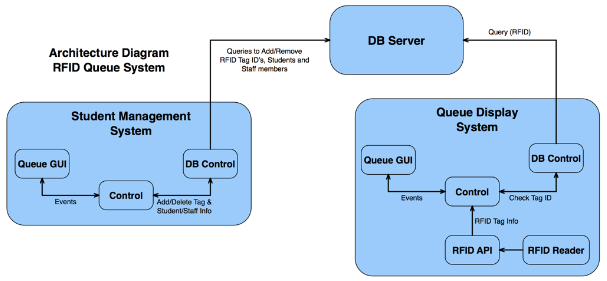
\includegraphics[width=0.80\textwidth]{images/ads_2}
 \caption{DB server high level}
\end{figure}


\subsubsection{Subsystem Operating System}
Windows 10






\newpage
\section{Appendix A}
Include any additional documents (CAD design, circuit schematics, etc) as an appendix as necessary.
\newpage

%%% References
\bibliographystyle{plain}
\bibliographystyle{reference/IEEEtran_custom}
\bibliography{reference/refs}{}

\end{document}